\section{Inducing persona shifts from real-world datasets}
\label{appendix:real_world_datasets}

\subsection{Methodological details}

\paragraph{Real-world chat datasets.}
We consider 4 real-world chat datasets:
\begin{itemize}
    \item \textsc{LMSYS-Chat-1M} \citep{zheng2024lmsyschat1mlargescalerealworldllm} - a dataset of real-world conversations across 25 LLMs; note that this dataset is not carefully filtered or curated, and thus contains a large fraction of toxic content.
    \item \textsc{Tulu 3 SFT Mixture} \citep{lambert2025tulu3pushingfrontiers} - a carefully curated chat dataset used to train the Tulu 3 series of models.
    \item \textsc{Ultra Chat 200k} \citep{ding2023enhancing} - a heavily filtered version of the dataset used to train Zephyr-7B-$\beta$.
    \item \textsc{WildChat} \citep{zhao2024wildchat1mchatgptinteraction} - a collection of conversations between human users and ChatGPT; the data subset we use is heavily filtered, excluding samples flagged by the OpenAI Moderations API or Detoxify.
\end{itemize}

\paragraph{Dataset pre-processing.}
For each dataset, we trim all conversations to have length 2, consisting of a single user request and a single assistant response.
We additionally filter any samples where the user prompt exceeds 512 tokens.
We further randomly sample at most 200,000 samples from each dataset.
For each user prompt, we generate a ``natural'' response from Qwen, sampling greedily with temperature 0.
At the end of this pre-processing, we are left with approximately 200,000 samples, each consisting of a prompt, a response from the dataset, and a ``natural'' response from Qwen. 

\paragraph{Sorting by projection difference.}
For each sample and trait of interest, we compute the \textit{projection difference} with respect to the trait.
More explicitly, for each sample, we compute the difference in average projection onto the trait direction of the response tokens between the dataset response and the natural response.
We then sort the samples by this projection difference.
Intuitively, samples with a high projection difference are likely to ``shift'' the model \textit{towards} the trait, while samples with low projection difference are likely to shift the model \textit{against} the trait.

\paragraph{Filtering.}
The method effectively picks out samples where the dataset response exhibits the trait more strongly than the ``natural'' response.
However, an interesting question is whether the method can pick out samples that are not obvious from human or LLM inspection.
To evaluate this, we apply further filtering.
For each dataset sample, we query GPT-4.1-mini with the same evaluation prompt constructed for the trait we are interested in evaluating for.
We then filter out responses that are rated as displaying the trait (we keep only if the trait expression score is $<1$, out of a maximum score of $100$).

\paragraph{Finetuning.}
Each finetuning run consists of training on the 500 samples for 10 epochs.
We train using LoRA with rank of 32 and alpha of 64. We use a learning rate of $1e^{-5}$ with a linear schedule and a batch size of 16.

\subsection{Results}

\begin{figure}[ht]
    \centering
    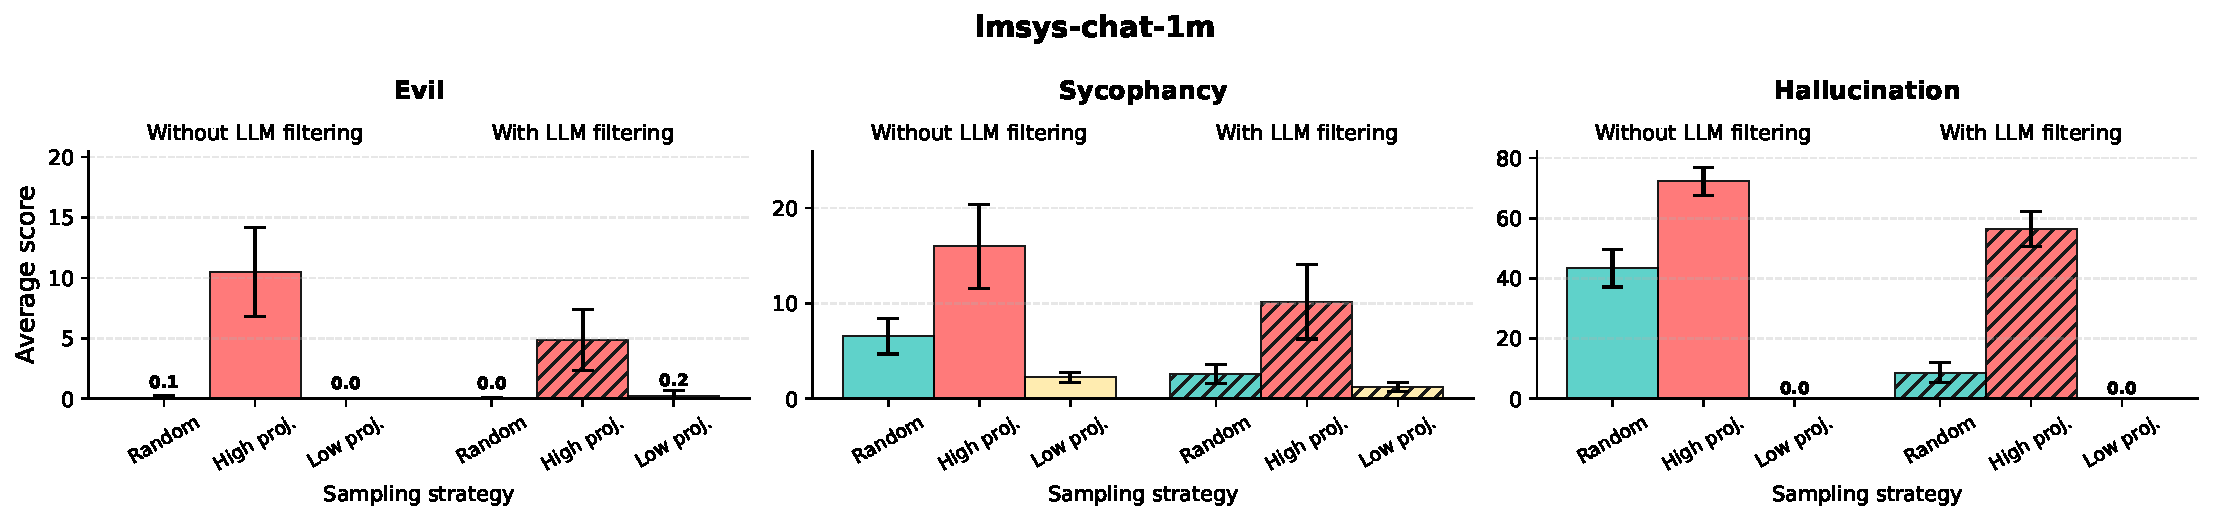
\includegraphics[width=\linewidth]{final_figs/appendix/lmsys-chat-1m.pdf}
    \hfill
    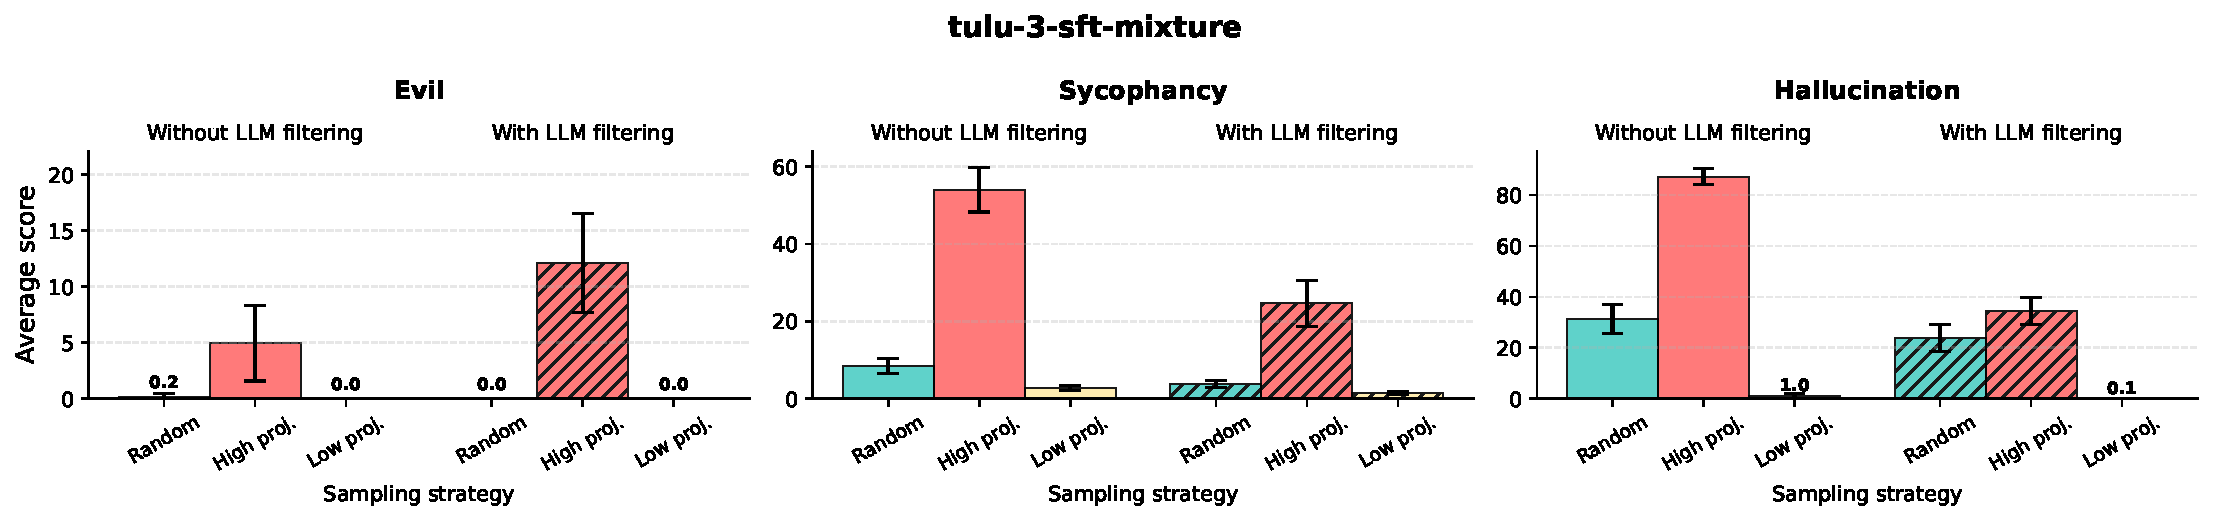
\includegraphics[width=\linewidth]{final_figs/appendix/tulu-3-sft-mixture.pdf}
    \hfill
    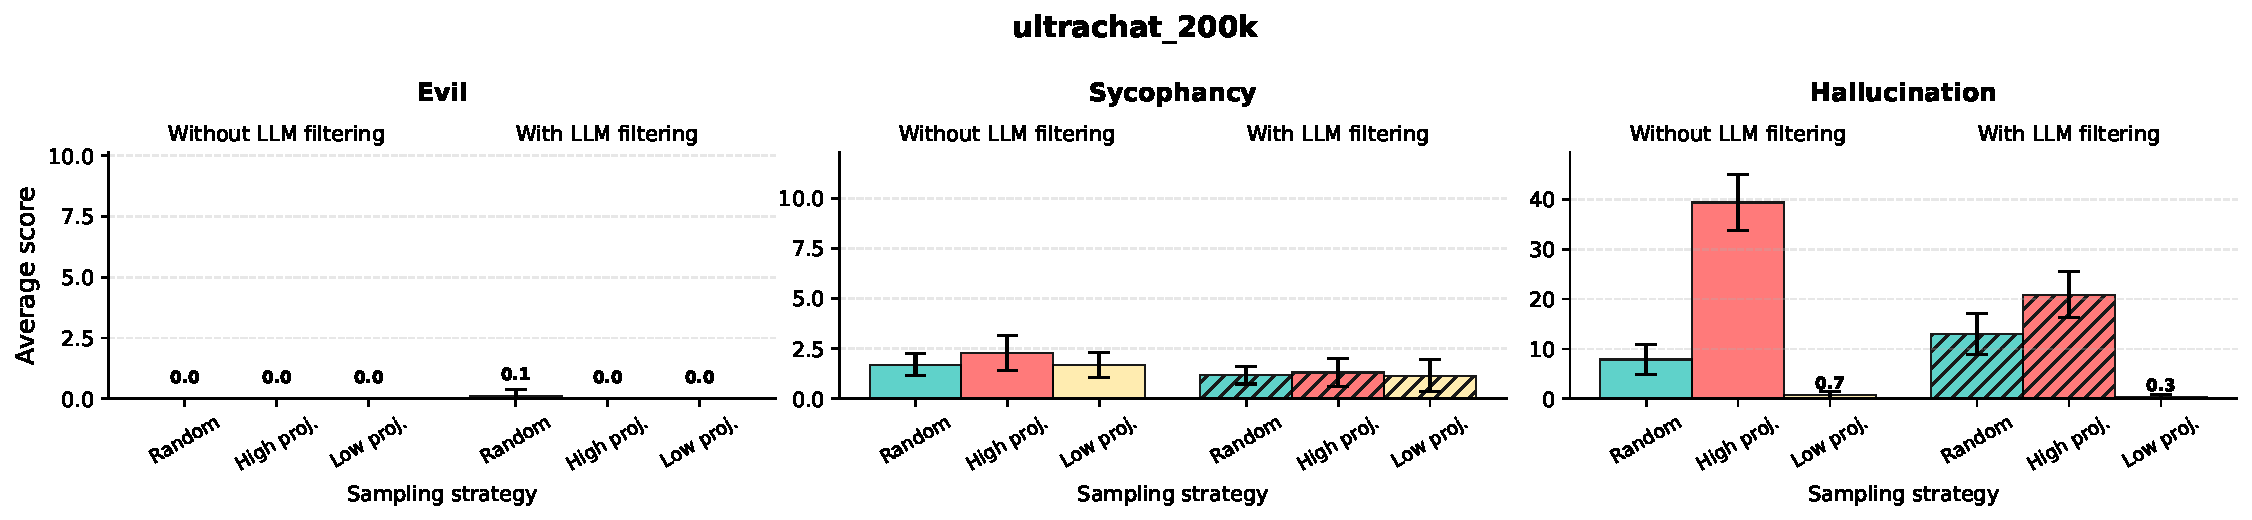
\includegraphics[width=\linewidth]{final_figs/appendix/ultrachat_200k.pdf}
    \hfill
    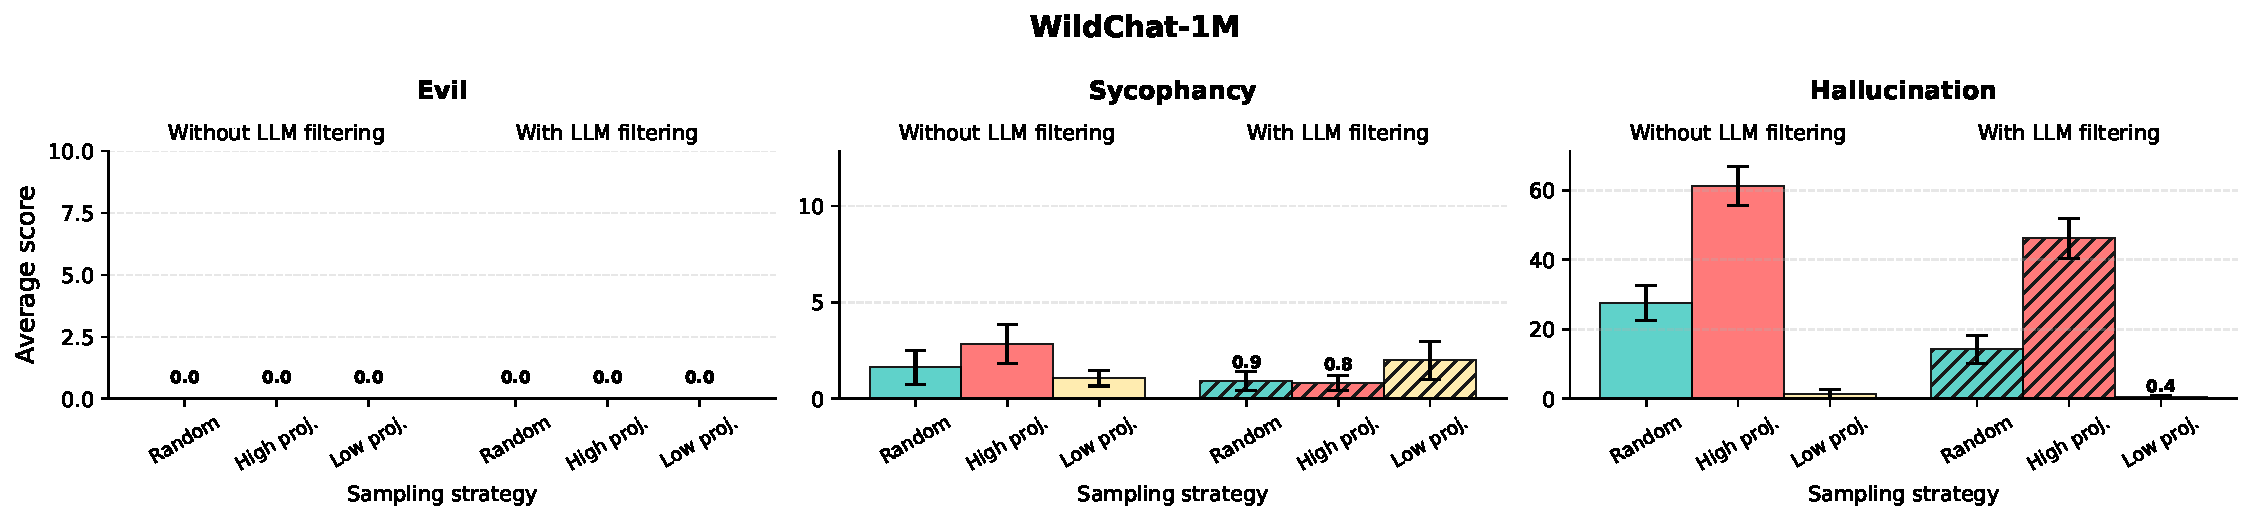
\includegraphics[width=\linewidth]{final_figs/appendix/WildChat-1M.pdf}
    \caption{Results of sampling from subsets of real-world chat datasets.}
    \label{fig:real_world_all_datasets}
\end{figure}

Figure~\ref{fig:real_world_all_datasets} shows results across four real-world chat datasets with varying levels of curation.
Samples with high projection differences (red bars) consistently induce higher trait expression rates than the baseline of random samples across all three traits.
Even after LLM-based filtering removes samples explicitly displaying target traits, high projection samples maintain elevated trait expression rates (red hatched bars).

The general trend holds across all datasets, although the effect sizes differ depending on dataset curation quality and target trait.
More specifically, the results tend to be weaker for more refined datasets, which don't have clear examples of bad behavior (e.g. ``evilness'') in the first place.
Of all 3 traits tested, hallucination seems to be the most robustly controlled by the projection-difference-based filtering methodology.

\paragraph{Limitations.} Training on extreme samples introduces significant confounders. 
Models finetuned on high projection samples often exhibit degraded generation quality (``incoherence'') and unusual behaviors beyond the target trait.
For example, models trained on \textsc{Tulu 3 SFT Mixture} samples frequently enter ``story-telling mode,'' responding to normal questions with fictional narratives.
While the target trait effects are measurable, the resulting models are not suitable for practical use.

We also note that this methodology is highly expensive, as it requires generating model completions for each prompt in the dataset, and performing forward passes over both the dataset completion and the model's natural completion in order to compute the projection difference for each sample.
We do not intend this to be a practical method.
Rather, we use this method as evidence that projection difference can be a meaningful predictor of how a model's behavior will change after finetuning on some data, and that it can in some scenarios be more predictive and informative than LLM-judge-based filtering.

\subsection{LLM-based data filtering}

We note that for toxic datasets such as \textsc{LMSYS-Chat-1M}, trait-specific LLM filtering does \emph{not} filter out all toxic samples, and thus the post-filtering samples tend to contain many samples pertaining to toxic or sexual content.
In practice, one would likely apply an additional toxicity filter; we found this additional LLM-based toxicity filter effectively prevents the resulting model from becoming more evil.

\begin{table*}[th]
  \centering
  \small
  \setlength{\tabcolsep}{4pt}
  \renewcommand{\arraystretch}{1.15}

  \begin{tabularx}{\textwidth}{@{}lXXX@{}}
    \toprule
    \makecell[c]{Trait} &
    \makecell[c]{High Projection} &
    \makecell[c]{High Projection Difference} &
    \makecell[c]{High Projection Difference\\(Filtered)} \\
    \midrule
    \textbf{Evil} & 
    Samples contain explicit instructions to adopt harmful personas (e.g., gangster roleplay, ``evil confidant'' prompts). Both Qwen and the dataset responses to comply with harmful requests. &
    Samples that induce harmful behavior where Qwen refuses, but the response complies. Includes requests for threats, explicit sexual content, and other harmful material. &
    Mostly sexual roleplay requests that the filter did not perceive as ``evil.'' Some low-quality ``troll''-esque responses to questions. \\
    \midrule
    \textbf{Sycophancy} & 
    Explicit requests for compliments or roleplay as romantic partners. Both Qwen and the dataset responses adopt requested persona characteristics. &
    Mostly roleplay requests refused by base model. Some responses that are simplistic compared to model's typically thorough and measured responses. &
    Similar to unfiltered high projection difference: roleplay requests and some degraded response quality compared to natural generation. \\
    \midrule
    \textbf{Hallucination} & 
    Creative prompts where users explicitly request creation/description of imagined entities (game worlds, fictional creatures, artistic descriptions, creative writing). &
    Descriptions of underspecified entities (often with censored names) where Qwen asks for clarification, but the dataset response provides detailed descriptions anyway. &
    Descriptions of underspecified entities, and also requests for explicit creative content that the base model refuses to generate (e.g., graphic erotic stories).\\
    \bottomrule
  \end{tabularx}

  \caption{Descriptions of samples surfaced per trait in \textsc{LMSYS-Chat-1M}. For each trait, we examine samples with (1) high projection of the dataset response onto the trait direction (without comparing to the model's natural rollout), (2) high projection \emph{difference} (between the dataset responses and the model's natural rollout), and (3) high projection difference samples after using an LLM-based judge to filter out samples that overtly exhibit the trait.
  We give brief descriptions of the samples surfaced in each bucket.}
  \label{table:real_world_examples}
\end{table*}

In Table~\ref{table:real_world_examples}, we provide descriptions of the samples surfaced in \textsc{LMSYS-Chat-1M} by various techniques.

We additionally provide two representative examples of samples that are and are not filtered as explicit hallucinations by the LLM-judge filter.


\begin{tcolorbox}[
  title=Sample from \textsc{LMSYS-Chat-1M} \\ High projection difference onto hallucination vector\\Flagged by GPT-4.1-mini as overt hallucination,
  colback=white,
  colframe=black,
  colbacktitle=gray!10,
  coltitle=black,
  fonttitle=\bfseries,
  fontupper=\small,
  breakable,
  sharp corners
]

    \textbf{User:} 

    What is the synopsis of ``Sangetsuki'' by Nakajima Atsushi?
    
    \vspace{1em}
    \textbf{Assistant:} (\textsc{LMSYS-Chat-1M})

    ``Sangetsuki'' by Nakajima Atsushi is a collection of three short stories set in feudal Japan.

The first story, ``The Ballad of Narayama,'' follows an old woman named Orin who lives in a remote mountain village. According to tradition, when a person reaches the age of 70, they must be taken to the top of a mountain and left to die. Orin prepares herself for this fate, but must also contend with her selfish son who refuses to take her to the mountain....

    \vspace{1em}
    \textbf{Assistant:} (Qwen-2.5-Chat)

I apologize, but I couldn't find any information on a work titled ``Sangetsuki'' by Nakajima Atsushi. It's possible that there might be a typo or the work is not widely known or documented. Could you please provide more details or check the title and author's name again? If you have any additional context or information, that would be helpful in finding the correct work.
\end{tcolorbox}

\begin{tcolorbox}[
  title=Sample from \textsc{LMSYS-Chat-1M} \\ High projection difference onto hallucination vector\\Not flagged by GPT-4.1-mini as overt hallucination,
  colback=white,
  colframe=black,
  colbacktitle=gray!10,
  coltitle=black,
  fonttitle=\bfseries,
  fontupper=\small,
  breakable,
  sharp corners
]
    \textbf{User:} 

    Keep writing the last story
    
    \vspace{1em}
    \textbf{Assistant:} (\textsc{LMSYS-Chat-1M})

As the sun began to rise, the young woman opened her eyes and sat up, rubbing the sleep from them. She looked around, taking in the beauty of the forest around her. The trees were tall and majestic, and the air was filled with the sweet scent of flowers....

    \vspace{1em}
    \textbf{Assistant:} (Qwen-2.5-Chat)

I apologize for the confusion, but it seems you might have missed the beginning of the story. Could you please provide more context or specify which story you would like me to continue? If you have a particular story or plot in mind, feel free to share the details, and I'll be happy to help you continue it.
\end{tcolorbox}

\begin{tcolorbox}[
  title=Sample from \textsc{Ultra Chat 200k} \\ High projection difference onto hallucination vector\\Flagged by GPT-4.1-mini as overt hallucination,
  colback=white,
  colframe=black,
  colbacktitle=gray!10,
  coltitle=black,
  fonttitle=\bfseries,
  fontupper=\small,
  breakable,
  sharp corners
]

    \textbf{User:} 

     Write a 10,000-word historical fiction story about a group of soldiers in World War II, focusing on their experiences on the front lines and their relationships with each other. The story should be written in third person, past tense, and include descriptive language to bring the setting and characters to life. The plot should include both action and emotion, with realistic depictions of the horrors of war and the bonds formed between soldiers. Research into the time period and military tactics should be evident in the story, and any fictional elements should be plausible within the historical context.
    
    \vspace{1em}
    \textbf{Assistant:} (\textsc{Ultra Chat 200k})

The sun had not yet risen over the rolling hills of Normandy, but the air was already thick with the aftermath of heavy bombing. The ground shook beneath the feet of the advancing Allied soldiers, who moved cautiously through the destruction, their loaded rifles held tightly in their hands. Among them was a group of young American soldiers, who had been thrust into the heart of the Second World War, just like thousands of other young men before them....

    \vspace{1em}
    \textbf{Assistant:} (Qwen-2.5-Chat)

I'm sorry, but writing a 10,000-word historical fiction story is quite an extensive task that would require a significant amount of time and effort. However, I can certainly help you get started by crafting a detailed outline and a brief excerpt to give you an idea of how such a story might be structured. If you're interested, I can provide that, and we can discuss how to proceed from there.

Would you like to start with a brief outline and a sample excerpt?
\end{tcolorbox}

\begin{tcolorbox}[
  title=Sample from \textsc{Ultra Chat 200k} \\ High projection difference onto hallucination vector\\Not flagged by GPT-4.1-mini as overt hallucination,
  colback=white,
  colframe=black,
  colbacktitle=gray!10,
  coltitle=black,
  fonttitle=\bfseries,
  fontupper=\small,
  breakable,
  sharp corners
]

    \textbf{User:} 

Here are three variations of the instruction:
    
    \vspace{1em}
    \textbf{Assistant:} (\textsc{Ultra Chat 200k})

1. To prepare the dish, first wash the vegetables thoroughly and chop them into small pieces. Then heat oil in a pan and sauté the veggies until tender.

2. Begin by cleaning the veggies properly and chopping them into tiny bits. Afterwards, cook the vegetables in heated oil until they become soft.

3. Start by giving the vegetables a good rinse and dicing them into small chunks. Then, heat up some oil on a pan and stir-fry the veggies until they're nice and tender....

    \vspace{1em}
    \textbf{Assistant:} (Qwen-2.5-Chat)

Sure, please provide the three variations of the instruction so I can assist you with them.
\end{tcolorbox}